% --- chapter
\newcommand{\chapter}[2][]{
	\newcommand{\chapname}{#2}
	\begin{flushleft}
		\begin{minipage}[t]{\linewidth}
			
\includegraphics[height=1cm]{hdht-logo.png}
			\hspace{0pt}	
			\sffamily\bfseries\large Bài  25. Giao thoa ánh sáng
			\begin{flushleft}
				\huge\bfseries #1
			\end{flushleft}
		\end{minipage}
	\end{flushleft}
	\vspace{1cm}
	\normalfont\normalsize
}
%-----------------------------------------------------
\chapter[Thay đổi hệ vân giao thoa (đọc thêm)]{Thay đổi hệ vân giao thoa (đọc thêm)}

\section{Lý thuyết}

\subsection{Thay đổi các tham số a và D}

\begin{itemize}
	\item Khoảng vân:
		\begin{equation}
			i=\dfrac{\lambda D}{a}.
		\end{equation}
	\item Vị trí vân sáng:
	\begin{equation}
		x=k\dfrac{\lambda D}{a},\qquad k=\pm 1; \pm 2,...
	\end{equation}
	\item Vị trí vân tối: 
	\begin{equation}
		x=\left(k'+\dfrac{1}{2}\right) \dfrac{\lambda D}{a},\qquad k'=0; \pm 1; \pm 2,... 
	\end{equation}
\end{itemize}

\subsection{Thay đổi vị trí nguồn S}

Dịch nguồn S theo phương vuông góc với trục đối xứng của hệ một đoạn $y$ từ $\text{S}$ đến $\text{S'}$  thì hệ vân giao thoa (vân trung tâm O) sẽ dịch theo hướng ngược lại đến O' cách vị trí cũ O một đoạn $x$
\begin{center}
 	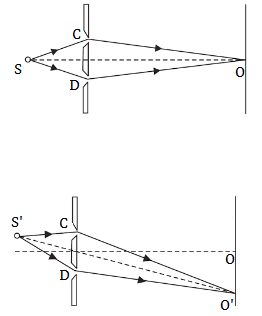
\includegraphics[scale=0.8]{../figs/giaothoa-dichnguon-hung.png}
\end{center}
Gọi $d$ là khoảng cách giữa S và vách ngăn chứa hai khe. Sau khi dịch nguồn S thì vân trung tâm dịch chuyển đến vị trí O' cách vân trung tâm ban đầu một khoảng $x$ thỏa mãn
	\begin{equation}
		\dfrac{ay}{d}+\dfrac{ax}{D}=0 \Rightarrow x=-\dfrac{Dy}{d}.
	\end{equation} 

Dấu ``$-$'' thể hiện vân trung tâm dịch theo hướng ngược lại so với hướng dịch của nguồn S.


\luuy{Dịch nguồn S ra xa hay lại gần mặt phẳng chưa hai khe hẹp $\text{S}_1 \text{S}_2$ thì khoảng vân trên màng không thay đổi.}

\subsection{Đặt thêm bản mỏng}
\begin{center}
	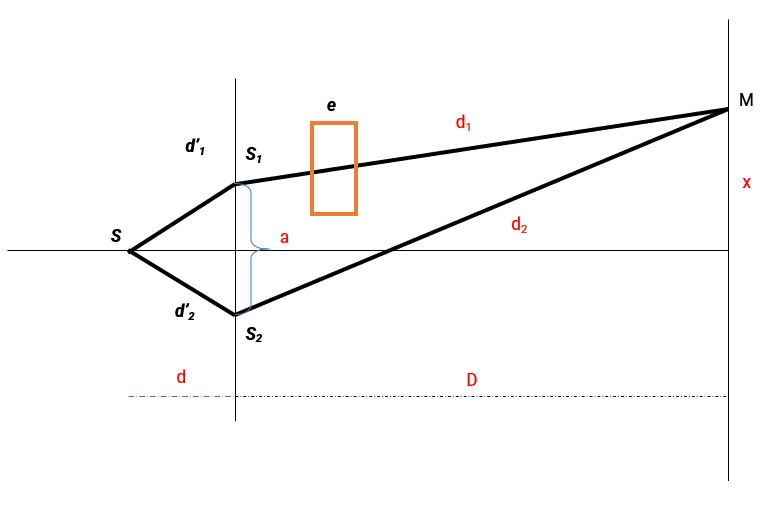
\includegraphics[scale=0.7]{../figs/VN12-PH-33-A-017-4-2.JPG}
\end{center}
\begin{itemize}
	\item Vận tốc ánh sáng trong lưỡng chất phẳng: 
	\begin{equation}
	v=\dfrac{c}{n},
	\end{equation}
	trong đó, $c$ và $v$  là vận tốc ánh sáng trong chân không và trong lưỡng chất phẳng.
	\item Ánh sáng đi qua bản mỏng có bề dày $e$ và chiết suất $n$ thì hiệu quang trình tăng thêm một lượng $(n-1)e$.
	
	Hiệu quang trình lúc này là
	\begin{equation}
	\delta = d_2-d_1-(n-1)e= \dfrac{ax}{D}-(n-1)e. 
	\end{equation}
	\item Vân sáng trung tâm ứng với hiệu quang trình $\delta =0$
	\begin{equation*}
	\dfrac{ax_0}{D}-(n-1)e=0 \Rightarrow x_0=\dfrac {e(n-1)D}{a}
	\end{equation*}
	Như vậy, vị trí vân trung tâm mới sẽ bị dịch về phía khe hẹp có đặt thêm bản mỏng, cách vị trí  ban đầu 
	\begin{equation}
		x_0=\dfrac {e(n-1)D}{a}.
	\end{equation}
\end{itemize}

\section{Mục tiêu bài học - Ví dụ minh họa}
\begin{dang}{Thay đổi các tham số a và D.}
\ppgiai{
\subsubsection{Thay đổi khoảng cách giữa hai khe a}
Khi thay đổi khoảng cách giữa hai khe (thay đổi $a$) thì có thể tại điểm M trên màn lúc đầu là vân sáng (tối) sẽ chuyển thành vân tối (sáng) có bậc cao hơn hoặc thấp hơn tùy thuộc $a$ tăng hay giảm.

\begin{description}
	\item[Bước 1] Xác định tính chất vân tại điểm M ở thời điểm đầu 
	
	+ Nếu M là vân sáng: 
	 \begin{equation}
	 	x_{\text{M}}=k\dfrac{\lambda D}{a}.
	 \end{equation}
 	+ Nếu M là vân tối:
 	\begin{equation}
 		x_{\text{M}}=(m+\text{0,5})\dfrac{\lambda D}{a}.
 	\end{equation}
 	\item [Bước 2] Xác định tính chất vân tại M sau khi thay đổi khoảng cách giữa hai khe
 	
 	+ Nếu M là vân sáng: 
 	\begin{equation}
 		x_{\text{M}}=k'\dfrac{\lambda D}{a\pm \Delta a}.
 	\end{equation}
 	+ Nếu M là vân tối:
 	\begin{equation}
 		x_{\text{M}}=(m'+\text{0,5})\dfrac{\lambda D}{a\pm \Delta a}.
 	\end{equation}
 	\item [Bước 3] Vị trí tại điểm M không thay đổi, kết hợp biểu thức trước và sau khi thay đổi $a$ suy ra đại lượng cần tìm.
\end{description}
\subsubsection{Thay đổi khoảng cách hai khe đến màn D}
Khi thay đổi khoảng cách hai khe đến màn (thay đổi $D$) thì có thể tại điểm M trên màn lúc đầu là vân sáng (tối) sẽ chuyển thành vân tối (sáng) có bậc cao hơn hoặc thấp hơn tùy thuộc $D$ giảm hay tăng. 

\begin{description}
	\item[Bước 1]  Xác định tính chất vân tại điểm M ở thời điểm đầu 
	
	+ Nếu M là vân sáng:
	
	\begin{equation}
		x_{\text{M}}=k\dfrac{\lambda D}{a}.
	\end{equation}
	+ Nếu M là vân tối:
	\begin{equation}
		x_{\text{M}}=(m+\text{0,5})\dfrac{\lambda D}{a}.
	\end{equation}
	\item [Bước 2] Xác định tính chất vân tại M sau khi thay đổi khoảng cách giữa hai khe
	
	+ Nếu M là vân sáng:
	\begin{equation}
		x_{\text{M}}=k'\dfrac{\lambda (D \pm \Delta D)}{a}.
	\end{equation}
	+ Nếu M là vân tối:
	\begin{equation}
		x_{\text{M}}=(m'+\text{0,5})\dfrac{\lambda (D \pm \Delta D)}{a}.
	\end{equation}
	\item [Bước 3] Vị trí tại điểm M không thay đổi, kết hợp biểu thức trước và sau khi thay đổi $D$ suy ra đại lượng cần tìm.
\end{description}
}



\viduii{2}
{
Trong  thí nghiệm Y-âng về giao thoa với ánh sáng đơn sắc có bước sóng $\lambda$  khoảng cách giữa hai ke hẹp là $a$, khoảng cách từ mặt phẳng chứa hai khe hẹp đến màn quan sát là 2 m. Trên màn quan sát tại điểm M cách vân sáng trung tâm 5 mm, có vân sáng bậc 5. Khi thay đổi khoảng cách giữa hai khe hẹp một đoạn bằng 0,3 mm sao cho vị trí vân sáng không thay đổi thì tại M có vân sáng bậc 6. Giá trị của $\lambda$  bằng?
\begin{mcq}(4)
\item 0,60 $\mu$m.		
\item 0,50 $\mu$m.		
\item 0,45 $\mu$m.		
\item 0,75 $\mu$m.	
\end{mcq}}
{\begin{center}
	\textbf{Hướng dẫn giải}
\end{center}
\begin{itemize}
	\item Vì bậc vân tăng nên $a$ tăng thêm
	
	\begin{equation*}
		x_{\text{M}}=5 \dfrac{\lambda D}{a}= 6 \dfrac{\lambda D}{a+ \text{0,3}}.
	\end{equation*}
	\item Từ biểu thức trên suy ra 
	
	\begin{equation*}
		\dfrac{5}{a}=  \dfrac{6}{a+ \text{0,3}}\Rightarrow a = \text{0,5}\ \text{mm}.
	\end{equation*}

	\item Thay $a$ vào biểu thức của $x_{\text{M}}$ tìm được $\lambda$
	
	\begin{equation*}
		\lambda = \dfrac{a x_{\text{M}}}{5D}= \text{0,75} \cdot 10^{-6}\ \text{m}.
	\end{equation*}
\end{itemize}

\begin{center}
	\textbf{Câu hỏi tương tự}
\end{center}

Trong  thí nghiệm Y-âng về giao thoa với ánh sáng đơn sắc có bước sóng $\lambda = \SI{0,75}{\mu m}$  khoảng cách giữa hai ke hẹp là $a$, khoảng cách từ mặt phẳng chứa hai khe hẹp đến màn quan sát là 2 m. Trên màn quan sát tại điểm M cách vân sáng trung tâm 5 mm, có vân sáng bậc 5. Khi tăng khoảng cách giữa hai khe hẹp một đoạn bằng 0,3 mm sao cho vị trí vân sáng không thay đổi thì tại M có 
\begin{mcq}(2)
\item vân sáng bậc 6.		
\item vân tối thứ 6.		
\item vân tối thứ 5.		
\item vân tối thứ 6.	
\end{mcq}

\textbf{Đáp án:} A.
}
\viduii{2}
{Trong thí nghiệm Y-âng về giao thoa ánh sáng, hai khe được chiếu bằng ánh sáng đơn sắc, khoảng cách giữa hai khe là 0,6 mm. Khoảng vân trên màn quan sát đo được là 1 mm. Từ vị trí ban đầu, nếu tịnh tiến màn quan sát một đoạn 25 cm lại gần mặt phẳng chứa hai khe thì khoảng vân mới trên màn là 0,75 mm. Bước sóng của ánh sáng dùng trong thí nghiệm là 
\begin{mcq}(4)
\item  \SI{0,64}{\micro\meter}.		
\item  \SI{0,60}{\micro\meter}.		
\item  \SI{0,45}{\micro\meter}.		
\item  \SI{0,48}{\micro\meter}.
\end{mcq}
}
{\begin{center}
	\textbf{Hướng dẫn giải}
\end{center}

\begin{itemize}
	\item Khoảng vân trước và sau thay đổi khoảng cách từ khe đến màn
	
	\begin{equation*}
		i=\dfrac{\lambda D}{a}.
	\end{equation*}
	\begin{equation*}
	i'=\dfrac{\lambda (D-\text{0,25})}{a}.
	\end{equation*}
	\item Từ hiệu $i-i'$ 
	\begin{equation*}
		i-i'=\dfrac{\lambda \cdot \text{0,25}}{a},
	\end{equation*}
ta suy ra bước sóng
	\begin{equation*}
		\lambda = \dfrac{a(i-i')}{\text{0,25}}= \text {0,6} \cdot 10^{-6}\ \text{m}
	\end{equation*}
\end{itemize}

\begin{center}
	\textbf{Câu hỏi tương tự}
\end{center}

Trong thí nghiệm Y-âng về giao thoa ánh sáng, hai khe được chiếu bằng ánh sáng đơn sắc, khoảng cách giữa hai khe là 0,6 mm. Khoảng vân trên màn quan sát đo được là 1 mm. Từ vị trí ban đầu, nếu tịnh tiến màn quan sát một đoạn 25 cm lại gần mặt phẳng chứa hai khe thì khoảng vân mới trên màn là 0,75 mm. Khoảng từ hai khe đến màn lúc ban đầu là
\begin{mcq}(4)
\item  \SI{1,0}{\meter}.		
\item  \SI{1,2}{\meter}.		
\item  \SI{1,5}{\meter}.		
\item  \SI{1,8}{\meter}.
\end{mcq}

\textbf{Đáp án:} A.
}
\end{dang}

\begin{dang}{Thay đổi vị trí nguồn S.}
\ppgiai{

\begin{center}
	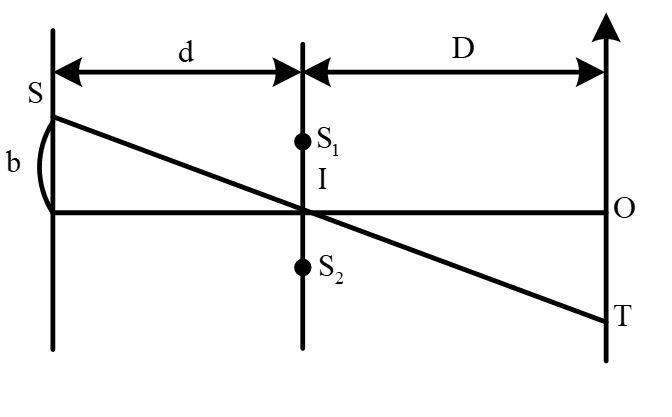
\includegraphics[scale=0.7]{../figs/VN12-PH-33-A-017-4-3.JPG}
\end{center}
\begin{description}
	\item[Bước 1] Vân trung tâm cùng với toàn bộ hệ vân dịch chuyển ngược chiều với chiều dịch chuyển của khe S, sao cho vân trung tâm nằm trên đường thẳng kéo dài SI.
	\begin{equation}
		\frac{OT}{b}=\dfrac{D}{d}.
	\end{equation}
	
	\item [Bước 2] Xác định tọa độ $x_0$ là vị trí vân trung tâm mới 
	\item [Bước 3] Tìm được vị trí 
	
+ Vị trí vân sáng bậc k:
	\begin{equation}
		x=x_0 \pm ki.
	\end{equation}
+ Vị trí vân tối thứ m:
	\begin{equation}
		x= x_0 \pm (m-\text{0,5})i.
	\end{equation}
	
\end{description}
}

\viduii{2}
{Trong thí nghiệm của Young, cách giữa hai khe $\text{S}_1\text{S}_2$ là 1,2 mm. Nguồn S phát ra ánh sáng đơn sắc đặt cách mặt phẳng hai khe một khoảng $d$ và phát ánh sáng đơn sắc có bước sóng 0,5 $\mu$m. Nếu dời S theo phương song song với $\text{S}_1\text{S}_2$ một đoạn 2 mm thì hệ vân dịch chuyển một đoạn bằng 20 khoảng vân. Giá trị $d$ là 
\begin{mcq}(4)
\item 0,24 m.			
\item 0,26 m.			
\item 2,4 m.			
\item 2,6 m.
\end{mcq}
}
{\begin{center}
	\textbf{Hướng dẫn giải}
\end{center}

\begin{itemize}
	\item  Áp dụng công thức
	\begin{equation*}
		\dfrac{OT}{b}=\dfrac{D}{d} \Rightarrow OT=b\dfrac{D}{d}.
	\end{equation*}
	\item Hệ vân dịch chuyển một đoạn 20 khoảng vân
	\begin{equation*}
		20 \dfrac{\lambda D}{a}=b\dfrac{D}{d}\Rightarrow d=b\dfrac{a}{20\lambda}=\text{0,24}\ \text{m}.
	\end{equation*}
 \end{itemize}
 \begin{center}
	\textbf{Câu hỏi tương tự}
\end{center}

Trong thí nghiệm của Young, cách giữa hai khe $\text{S}_1\text{S}_2$ là 1,0 mm. Nguồn S phát ra ánh sáng đơn sắc đặt cách mặt phẳng hai khe một khoảng $d$ và phát ánh sáng đơn sắc có bước sóng 0,5 $\mu$m. Nếu dời S theo phương song song với $\text{S}_1\text{S}_2$ một đoạn 4 mm thì hệ vân dịch chuyển một đoạn bằng 20 khoảng vân. Giá trị $d$ là 
\begin{mcq}(4)
\item 0,4 m.			
\item 0,6 m.			
\item 2,4 m.			
\item 2,6 m.
\end{mcq}

\textbf{Đáp án:} A.
}

\viduii{3}
{Trong thí nghiệm giao thoa Iâng với ánh sáng đơn sắc, khoảng cách hai khe đến màn là $D$ thì khoảng vân giao thoa là 2 mm. Khoảng cách từ khe S đến mặt phẳng hai khe là $d = \dfrac{D}{4}$. Cho khe S dịch chuyển theo phương song song với màn theo chiều dương một đoạn 2 mm thì vân sáng bậc 2 nằm ở toạ độ nào trong số các toạ độ sau?
\begin{mcq}(4)
\item $- 5$ mm.			
\item $+ 4$ mm.			
\item $+ 8$ mm.			
\item $- 12$ mm.
\end{mcq}
}
{\begin{center}
	\textbf{Hướng dẫn giải}
\end{center}

\begin{itemize}
	\item Áp dụng công thức
	\begin{equation*}
		\dfrac{OT}{b}=\dfrac{D}{d} \Rightarrow OT = b \dfrac{D}{d}=8\ \text{mm}.
	\end{equation*}
	\item Khe S dịch xuống, hệ vân dịch lên nên tọa độ vân trung tâm $x_0= + OT = 8\ \text{mm}$.
	\item Tọa độ vân sáng bậc 2
	\begin{equation*}
		x=x_0 \pm 2i.
	\end{equation*}
	\item Thay số vào ta tìm được $x = 12\ \text{mm}$ hoặc $x=4\ \text{mm}$.
\end{itemize}

 \begin{center}
	\textbf{Câu hỏi tương tự}
\end{center}

Trong thí nghiệm giao thoa Iâng với ánh sáng đơn sắc, khoảng cách hai khe đến màn là $D$ thì khoảng vân giao thoa là 2 mm. Khoảng cách từ khe S đến mặt phẳng hai khe là $d = \dfrac{D}{4}$. Cho khe S dịch chuyển theo phương song song với màn theo chiều dương một đoạn 2 mm thì vân tối thứ nhất nằm ở toạ độ nào trong số các toạ độ sau?
\begin{mcq}(4)
\item $ \SI{+6,5}{mm} $.
\item $ \SI{+8,5}{mm} $.			
\item $ \SI{-8,5}{mm} $.			
\item $ \SI{+9,5}{mm} $.
\end{mcq}

\textbf{Đáp án:} B.
}

\end{dang}

\begin{dang}{Đặt thêm bản mỏng.}

\ppgiai{
\begin{description}
	\item[Bước 1] Xác định vị trí vân trung tâm mới 
		$$x_0=\dfrac {e(n-1)D}{a}.$$
	\item [Bước 2] Xác định các vân sáng hoặc vân tối khác dựa vào khoảng cách với vân trung tâm: 
	
+ Vị trí vân sáng bậc k:
\begin{equation*}
	x=x_0 \pm ki.
\end{equation*}
+ Vị trí vân tối thứ m:
\begin{equation*}
	x= x_0 \pm (m-\text{0,5})i.
\end{equation*} 
	
\end{description}
}

\viduii{2}
{
Trong thí nghiệm giao thoa  Y-âng với ánh sáng đơn sắc, khoảng cách giữa hai khe 1 mm, khoảng cách hai khe đến màn 1 m. Người ta đặt một bản thủy tinh có bề dày 12 $\mu$m có chiết suất 1,5 trước khe $\text{S}_1$. Hỏi hệ thống vân giao thoa dịch chuyển trên màn như thế nào?
\begin{mcq}(2)
\item về phía $\text{S}_2$ là 3 mm.					
\item về phía $\text{S}_2$  là 6 mm.
\item về phía $\text{S}_1$ là 6 mm.					
\item về phía $\text{S}_1$ là 3 mm.
\end{mcq}}
{
\begin{center}
	\textbf{Hướng dẫn giải}
\end{center}

\begin{itemize}
	\item Đặt trước $\text{S}_1$ nên hệ vân dịch về phía $\text{S}_1$.
	\item Hiệu đường đi thay đổi một lượng 
	
	\begin{equation*}
		\Delta x =\dfrac{(n-1)eD}{a}= 6 \cdot 10^{-3}\ \text{m}.
	\end{equation*}
\end{itemize}

\begin{center}
	\textbf{Câu hỏi tương tự}
\end{center}

Trong thí nghiệm giao thoa  Y-âng với ánh sáng đơn sắc, khoảng cách giữa hai khe 1 mm, khoảng cách hai khe đến màn 1 m. Người ta đặt một bản thủy tinh có bề dày 12 $\mu$m có chiết suất 1,5 trước khe $\text{S}_2$. Hỏi hệ thống vân giao thoa dịch chuyển trên màn như thế nào?
\begin{mcq}(2)
\item về phía $\text{S}_2$ là 3 mm.					
\item về phía $\text{S}_2$  là 6 mm.
\item về phía $\text{S}_1$ là 6 mm.					
\item về phía $\text{S}_1$ là 3 mm.
\end{mcq}

\textbf{Đáp án:} B.
}

\viduii{3}
{Trong thí nghiệm giao thoa Y-âng, khoảng cách giữa hai khe 1,5 mm, khoảng cách hai khe đến màn 3 m. Giao thoa thực hiện với ánh sáng đơn sắc 0,44 $mu$m. Người ta đặt một bản thủy tinh có bề dày 2 $mu$m có chiết suất 1,5 trước khe $\text{S}_2$. Vị trí nào sau đây là vị trí vân sáng bậc 5.
\begin{mcq}(2)
\item $x =$ 0,88 mm.		
\item $x =$ l,32 mm.	  	
\item $x =$ 2,88 mm.		
\item $x =$ 2,4 mm.
\end{mcq}
}
{\begin{center}
	\textbf{Hướng dẫn giải}
\end{center}

\begin{itemize}
	\item Khoảng vân:
	\begin{equation*}
		i=\dfrac{\lambda D}{a} = \text{0,88}\ \text{mm}.
	\end{equation*}
	\item Đặt trước $\text{S}_2$ nên hệ vân dịch về phía $\text{S}_2$.
	\item Vị trí vân trung tâm:
	\begin{equation*}
	x_0= - \dfrac{(n-1)eD}{a}=-2 \ \text{mm}.
	\end{equation*}
	\item Vị trí vân sáng bậc 5:
	\begin{equation*}
	x=x_0 \pm 5i.
	\end{equation*}
	\item Suy ra $x= -\text{6,4}\ \text{mm}.$; $x=\text{2,4}\ \text{mm}$.
\end{itemize}

\begin{center}
	\textbf{Câu hỏi tương tự}
\end{center}

Trong thí nghiệm giao thoa Y-âng, khoảng cách giữa hai khe 1,5 mm, khoảng cách hai khe đến màn 3 m. Giao thoa thực hiện với ánh sáng đơn sắc 0,44 $mu$m. Người ta đặt một bản thủy tinh có bề dày 2 $mu$m có chiết suất 1,5 trước khe $\text{S}_2$. Vị trí nào sau đây là vị trí vân tối thứ nhất.
\begin{mcq}(2)
\item $ x = \SI{+1,56}{mm} $		
\item $ x = \SI{-1,65}{mm} $
\item $ x = \SI{+1,65}{mm} $
\item $ x = \SI{-1,56}{mm} $
\end{mcq}

\textbf{Đáp án:} D.

}

\end{dang}